\documentclass[letterpaper, 12pt]{article}

\usepackage{graphicx}
\usepackage{longtable}
\usepackage{rotating}
\usepackage{dcolumn}
\usepackage{listings}

% Code listing commands
\lstset{language=R,
basicstyle=\scriptsize\ttfamily,
commentstyle=\ttfamily,
numbers=left,
numberstyle=\footnotesize,
stepnumber=1,
numbersep=5pt,
showspaces=false,
showstringspaces=false,
showtabs=false,
frame=single,
tabsize=2,
captionpos=b,
breaklines=true,
breakatwhitespace=false,
title=\lstname,
escapeinside={},
keywordstyle={},
morekeywords={}
}

\begin{document}
\title{ARE213 Problem Set \#1B}
\author{Peter Alstone \& Frank Proulx}
\maketitle

\section{Problem \#1}
\subsection{Part A}
\emph{Under the assumption of random assignment conditional on the observables, what are the sources of misspecification bias in the estimates generated by the linear model estimated in Problem Set 1a?}

\paragraph{Wrong functional form.}
In Problem Set 1A we used linear (i.e., $ y = \beta x + \epsilon$) estimators to make ``corrections'' while the true functional form of the relationships between the covariates we included in the modern were certainly not linear.  By imposing a linear function on a non-linear data generating process (described by the CEF), we introduce misspecification bias in the model.  

\paragraph{Omitted Variables Bias.}  We were able to use variables included in the dataset in our linear model, but not the unobserved variables that may be important for control.  If omitted variables exist that both determine outcomes related to birth weight and are correlated with smoking status we will over- or under-estimate the effect (depending on the characteristics of the omission).   


\subsection{Part B}
\emph{Now, consider a series estimator. Estimate the smoking effects using a flexible functional form for the control variables (e.g., higher order terms and interactions). What are the benefits and drawbacks to this approach?}

We can attempt to reduce the magnitude of the first source of bias mentioned above (Functional Form) by introducing non-parametric series estimators as a replacement for linear regression.  

\section{Problem \#2}

The Propensity Score Method (PSM) uses a ``surrogate'' normalized metric (p-score) as a replacement for the observable controls that would normally be used to condition the estimates of a treatment response to the variable in question.  The p-score is defined as a normalized score that represents the likelihood a sample selects into treatment conditioned on observables.  Because it collapses all the dimensions into a 0:1 continuum PSM avoids the curse of dimensionality encountered with large nonparametric regression models, where it can be difficult to find neighbors or ``bandwidth-mates'' in n-dimensional space.  

\subsection{Part A}

To calculate the propensity score, we estimated a logit model of mother's tobacco use (0=non-smoker, 1=smoker) as determined by the predetermined covariates shown in Table \ref{tab:propensities}. Model \#1 shows the full model using all of the covariates suspected to be predetermined. Model \#2 is a reduced form of the same model, preserving just those covariates that were significant at the 1\% level in Model \#1. 

\let\clearpage\relax
 \documentclass{article}
\usepackage{dcolumn}

\begin{document}

% Table created by stargazer v.4.5.1 by Marek Hlavac, Harvard University. E-mail: hlavac at fas.harvard.edu
% Date and time: Wed, Oct 16, 2013 - 06:01:58 PM
% Requires LaTeX packages: dcolumn 
\begin{table}[!htbp] \centering 
  \caption{Logistic function coefficients for propensity score models} 
  \label{tab:propensities} 
\begin{tabular}{@{\extracolsep{5pt}}lD{.}{.}{-3} D{.}{.}{-3} } 
\\[-1.8ex]\hline 
\hline \\[-1.8ex] 
\\[-1.8ex] & \multicolumn{2}{c}{Mother Tobacco-Use Status} \\ 
\\[-1.8ex] & \multicolumn{1}{c}{(1)} & \multicolumn{1}{c}{(2)}\\ 
\hline \\[-1.8ex] 
 Mother's Race not White or Black & -1.956^{***} & -1.954^{***} \\ 
  & (0.134) & (0.133) \\ 
  & & \\ 
 Mother's Years of Education & -0.817^{***} & -0.818^{***} \\ 
  & (0.028) & (0.028) \\ 
  & & \\ 
 Marital status & -0.205^{***} & -0.204^{***} \\ 
  & (0.005) & (0.005) \\ 
  & & \\ 
 Father's age & -1.256^{***} & -1.251^{***} \\ 
  & (0.022) & (0.021) \\ 
  & & \\ 
 Father's Years of Education & 0.029^{***} & 0.030^{***} \\ 
  & (0.002) & (0.001) \\ 
  & & \\ 
 Father Mexican & -0.131^{***} & -0.131^{***} \\ 
  & (0.005) & (0.005) \\ 
  & & \\ 
 Father Puerto Rican & -1.961^{***} & -1.957^{***} \\ 
  & (0.173) & (0.173) \\ 
  & & \\ 
 Father Cuban & -1.267^{***} & -1.268^{***} \\ 
  & (0.058) & (0.058) \\ 
  & & \\ 
 Father Central or South American & -0.567 & -0.567 \\ 
  & (0.364) & (0.364) \\ 
  & & \\ 
 Father Race Other or Unknown Hispanic & -1.933^{***} & -1.932^{***} \\ 
  & (0.205) & (0.205) \\ 
  & & \\ 
 Plurality of Infant & -0.890^{***} & -0.889^{***} \\ 
  & (0.120) & (0.120) \\ 
  & & \\ 
 Sex of Infant & -0.148^{***} &  \\ 
  & (0.054) &  \\ 
  & & \\ 
 Mother's age & -0.019 &  \\ 
  & (0.017) &  \\ 
  & & \\ 
 dmage & 0.003 &  \\ 
  & (0.002) &  \\ 
  & & \\ 
 Constant & 2.873^{***} & 2.707^{***} \\ 
  & (0.088) & (0.064) \\ 
  & & \\ 
\textit{N} & \multicolumn{1}{c}{114,610} & \multicolumn{1}{c}{114,610} \\ 
Log Likelihood & \multicolumn{1}{c}{-44,310.690} & \multicolumn{1}{c}{-44,315.790} \\ 
Akaike Inf. Crit. & \multicolumn{1}{c}{88,651.370} & \multicolumn{1}{c}{88,655.580} \\ 
\hline 
\hline \\[-1.8ex] 
\textit{Notes:} & \multicolumn{2}{r}{$^{***}$Significant at the 1 percent level.} \\ 
 & \multicolumn{2}{r}{$^{**}$Significant at the 5 percent level.} \\ 
 & \multicolumn{2}{r}{$^{*}$Significant at the 10 percent level.} \\ 
\normalsize 
\end{tabular} 
\end{table} 
\end{document}



To test whether the propensity scores predicted by these two models are significantly different  we perform a likelihood ratio test between  the full and reduced model. This test yields the following output:

%Likelihood ratio test for MLE method 
Chi-squared 3 d.f. =  10.21274 , P value =  0.01684173 



NOTE from class: including insignificant terms can be beneficial in terms of getting better fit (by reducing 



\subsection{Part B}

This estimation assumes unconfoundedness. and conditional independence

% SECTION BELOW WAS RESULTING IN ERRORS on TeX compilation...commented out for now

%

% Table created by stargazer v.4.0 by Marek Hlavac, Harvard University. E-mail: hlavac at fas.harvard.edu
% Date and time: Thu, Oct 17, 2013 - 10:59:15
% Requires LaTeX packages: dcolumn 
\begin{table}[!htbp] \centering 
  \caption{Model of effects of tobacco use on birthweight using propensity score as a control} 
  \label{tab:propensitymodel} 
\footnotesize 
\begin{tabular}{@{\extracolsep{5pt}}lD{.}{.}{-3} } 
\\[-1.8ex]\hline 
\hline \\[-1.8ex] 
\\[-1.8ex] & \multicolumn{1}{c}{Mother Tobacco-Use Status} \\ 
\hline \\[-1.8ex] 
 Delta1 & -241.076^{***} \\ 
  & (16.738) \\ 
  & \\ 
 Beta & -237.099^{***} \\ 
  & (9.180) \\ 
  & \\ 
 Delta2 & 90.427^{***} \\ 
  & (34.496) \\ 
  & \\ 
 Constant & 3,445.897^{***} \\ 
  & (3.022) \\ 
  & \\ 
\textit{N} & \multicolumn{1}{c}{114,610} \\ 
R$^{2}$ & \multicolumn{1}{c}{0.025} \\ 
Adjusted R$^{2}$ & \multicolumn{1}{c}{0.025} \\ 
Residual Std. Error & \multicolumn{1}{c}{577.939} \\ 
F Statistic & \multicolumn{1}{c}{963.616} \\ 
\hline 
\hline \\[-1.8ex] 
\textit{Notes:} & \multicolumn{1}{r}{$^{***}$Significant at the 1 percent level.} \\ 
 & \multicolumn{1}{r}{$^{**}$Significant at the 5 percent level.} \\ 
 & \multicolumn{1}{r}{$^{*}$Significant at the 10 percent level.} \\ 
\normalsize 
\end{tabular} 
\end{table} 



%The estimated average treatment effect is given by 
%\begin{equation*}
%\delta_1 + \delta_2 \overbar{p}(X_i)=-237.099 + (0.1594*90.427)=-222.69
%\end{equation*}

This suggests that (pursuant to these assumptions) the average effect of smoking on birthweight is a reduction of 223 grams.

\subsection{Part C}

We estimate the average treatment effect of smoking on birthweight to be 222 grams when using the reweighting approach. This approach involved taking a weighted average of all observations using the (normalized inverse) of the propensity score as a weighting factor. This is consistent with the estimate produced using the regression approach.

We estimate the average treatment on the treated to be % We still need to figure this out.

\subsection{Part D}
Here we estimate the density function with a kernel density estimator, using the density() function in R. We estimate the density function separately for the smoking and non-smoking members of the sample, and weight their responses with the propensity scores normalized to the subsample (e.g. $p(X_i)/\sum\limits{j=1}^{N_{smokers}}p(X_j)$)

We estimate the density function using the Epanechnikov kernel and bandwidths ranging from 15 grams to 50 grams in increments of 5 grams. Figure \ref{fig:kernel40} shows the density function estimated with a bandwidth of 40 grams. This bandwidth appears to be a good compromise between washing out some of the noise at lower bandwidths while preserving the underlying CEF.

\begin{figure}[h!]
   \centering
   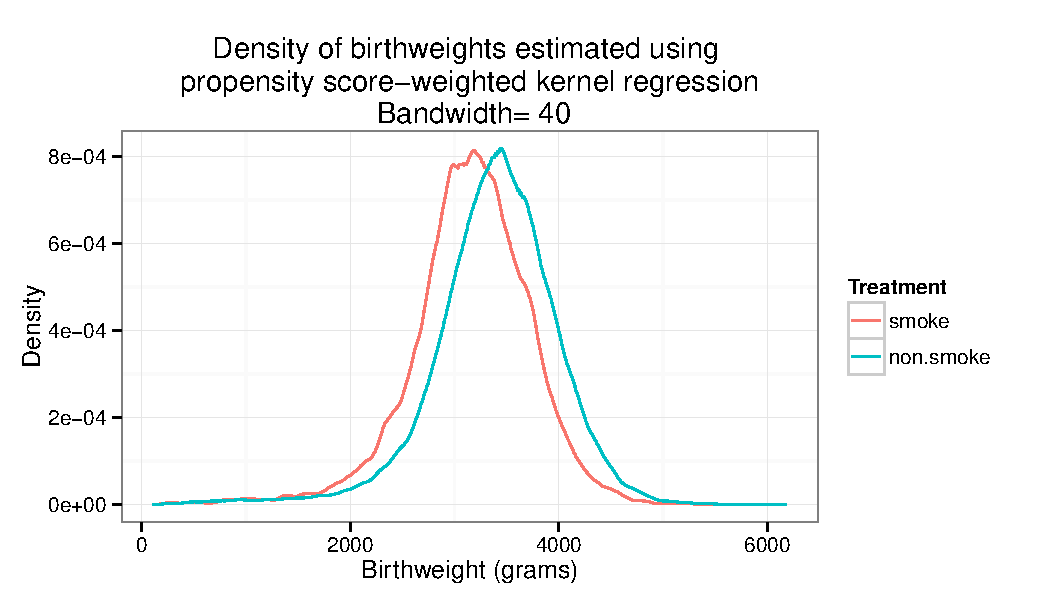
\includegraphics[width=4in]{img/kerndensity40.pdf} 
   \caption{Birthweight density function estimates produced using Epanechnikov kernel estimator for smokers and non-smokers.}
   \label{fig:kernel40}
\end{figure}

We also estimate the density at x=3000 grams by hand. We first calculate the average propensity score for both smokers and non-smokers with infants at 3000 grams. The dataset has 12 smokers and 47 non-smokers with infants born at this weight. The average propensity score for these smokers is 0.27 and for non-smokers it is 0.20. These values stand to reason- the people who have opted in to smoking in this class have been predicted as more likely to be smokers.



We used R to complete this assignment.  The code is below:

\lstinputlisting{ps1b.R}

\lstinputlisting{../util/are213-func.R}


\end{document}
